\documentclass[]{report}
\renewcommand\thesection{\arabic{section}}

\usepackage{listings}
\usepackage{xcolor}
\usepackage{graphicx}
\usepackage{tikz}
\usepackage{amsmath}
\usepackage{systeme,mathtools}
\usepackage{amsthm}
\usepackage{amssymb}
\usepackage{subfig}
\usepackage{caption}
\usepackage[english]{babel}
\newtheorem{theorem}{Theorem}
% Title Page
\title{Pollution of a drinking water reservoir}
\author{Masiero Niko}
\date{\today}


\begin{document}
\maketitle
\tableofcontents
\newpage
\section{Explanation of the problem}
We consider a squared reservoir that contains water flowing from $\Gamma_4$ to $\Gamma_2$ because of a difference of pressure. In the middle of this reservoir, in the region $C_1$, there is a pump. In the bounds $\Gamma_1$ and $\Gamma_3$ no water can flow because they are impervious.
\begin{figure}
\begin{center}
\begin{tikzpicture}
	\draw[black,thick] (-2,-2)--(2,-2);
	\draw[black,thick] (2,-2)--(2,2);
	\draw[black,thick] (2,2)--(-2,2);
	\draw[black,thick] (-2,2)--(-2,-2);
	\draw[black,thick] (-0.1,-0.1)--(0.1,-0.1);
	\draw[black,thick] (0.1,-0.1)--(0.1,0.1);
	\draw[black,thick] (0.1,0.1)--(-0.1,0.1);
	\draw[black,thick] (-0.1,0.1)--(-0.1,-0.1);
	\draw[black,thick] (-1.1,-1.1)--(-1.1,-0.9);
	\draw[black,thick] (-1.1,-0.9)--(-0.9,-0.9);
	\draw[black,thick] (-0.9,-0.9)--(-0.9,-1.1);
	\draw[black,thick] (-0.9,-1.1)--(-1.1,-1.1);
	\filldraw[black] (0,0) circle (0.01pt) node[anchor=west]{$C_1$};
	\filldraw[black] (-1,-1) circle (0.01pt) node[anchor=west]{$C_2$};
	\filldraw[black] (0,2) circle (0.01pt) node[anchor=south]{$\Gamma_3$};
	\filldraw[black] (0,-2) circle (0.01pt) node[anchor=north]{$\Gamma_1$};
	\filldraw[black] (2,0) circle (0.01pt) node[anchor=west]{$\Gamma_2$};
	\filldraw[black] (-2,0) circle (0.01pt) node[anchor=east]{$\Gamma_4$};
\end{tikzpicture}
\end{center}
\caption{Vertical view of the computational domain}
\label{init_prob}
\end{figure}
We consider the problem in which in the region $C_2$ ,positioned in the bottom-left quadrant (as we can see in the figure \ref{init_prob}), there is a pollution accident. Our goal is to model the stream of the water and the diffusion of the pollutant in order to see if it reach the pump and, in case, how much of the pollutant converge in the region $C_1$.
\section{Mathematical modelling}
The idea is to model the stream of the water as a Darcy flow, while the movement of the pollutant will be modelled with a diffusion-transport equation.
For the Darcy equation we consider homogeneous Neumann condition in $\Gamma_1$ and $\Gamma_3$ and for the diffusion-transport equation we consider that the pollutant can not reach the bounds $\Gamma_1$,$\Gamma_3$ and $\Gamma_4$ whereas we consider that in $\Gamma_2$ the pollutant concentration does not change following the stream.
The strong formulation for Darcy flow is:
\begin{equation}
\systeme{-\nabla p=k^{-1}\mathbf{u} \mbox{ in }\Omega,\nabla \cdot \mathbf{u}=f \mbox{ in } \Omega,p=p_{in} \mbox{ on }\Gamma_4,p=p_{out}\mbox{ on } \Gamma_2, \mathbf{u}\cdot \mathbf{n}=0 \mbox{ on } \Gamma_1\cup\Gamma_3}
\end{equation}
with $k=1$ defined as the permeability coefficient and $f$ such that
\begin{equation}
	f(x)=\begin{cases}
	-1000& \mbox{ if }x\in C_1\\
	0& \mbox{ otherwise}
	\end{cases}
\end{equation}
For the diffusion-transport equation the strong form is:
\begin{equation}
\systeme{-\nu\Delta c+\mathbf{u}\cdot \nabla c=g \mbox{ in } \Omega,c=0 \mbox{ on }\Gamma_1\cup\Gamma_3\cup\Gamma_4,\nu\nabla c\cdot\mathbf{n}=0 \mbox{ on }\Gamma_2}
\end{equation}
with $\nu=0.05$ and $g$ such that
\begin{equation}
g(x)=\begin{cases}
1000& \mbox{ if }x\in C_2\\
0& \mbox{ otherwise}
\end{cases}
\end{equation}
\subsection{Weak form of the problem}\label{ContWF}
The idea is to transform our equations in two variational problems of this type:
\begin{equation}
	\mbox{Find }\mathbf{u}\in V\mbox{ and }p\in Q\mbox{ such that}
	\systeme{a(\mathbf{u};\mathbf{v})-b(q;\mathbf{u})=F_1(\mathbf{v}),b(p;\mathbf{v})=F_2(q)}
	,\forall v \in V \mbox{ } \forall q \in Q
	\label{mixed}
\end{equation}
and
\begin{equation}
	\mbox{Find }c\in W\mbox{ such that }
	\tilde{a}(c,b)=G(b), \forall b\in W
	\label{diff_transp}
\end{equation}
In order to identify all these forms and space we need to look at the strong form, doing this we can suppose that:
\begin{equation}
	a(u,v)=\int_\Omega k^{-1}\mathbf{u}\mathbf{v}
	\label{bil_a}
\end{equation}
\begin{equation}
	b(q,\mathbf{u})=\int_\Omega q\cdot div(\mathbf{u})
\end{equation}
\begin{equation}
F_1(\mathbf{v})=\int_{\Gamma_2} p_{out} \mathbf{v}\cdot \mathbf{n} +\int_{\Gamma_4} p_{in} \mathbf{v}\cdot \mathbf{n}
\end{equation}
\begin{equation}
F_2(q)=\int_\Omega fq
\end{equation}
\begin{equation}
\tilde{a}(c,b)=\int_\Omega \nu\nabla c\nabla b+(\mathbf{u}\cdot \nabla c) b
\label{a_tilde}
\end{equation}
\begin{equation}
G(b)=\int_\Omega gb
\label{G}
\end{equation}
  and a sufficient condition for $\mathbf{u}$ will be $\mathbf{u}\in H_{\Gamma_1\cup\Gamma_3}(div,\Omega)=\{\mathbf{u}\in H(div,\Omega):\mathbf{u}\cdot\mathbf{n}|_{\Gamma_1\cup\Gamma_3}=0\}=V$. Now we are looking for a suitable space where $p$ could lie, we can suppose $p \in Q\subseteq L^2(\Omega)$. This space $Q$ will be such that the application  $div:V\longrightarrow Q$ is surjective.
\begin{theorem}
	If $V=H_{\Gamma_1\cup\Gamma_3}(div,\Omega)$ and $Q=L^2(\Omega)$ then the application
	\begin{equation*}
	div:V\longrightarrow Q
	\end{equation*}
	is surjective
\end{theorem}
\begin{proof}
	We consder the auxiliary problem
	\begin{equation*}
		\systeme{\Delta \mathbf{u}=h \mbox{ in } \Omega, \partial_n \mathbf{u}=0 \mbox{ on } \Gamma_1\cup\Gamma_3}
	\end{equation*}
	with $h \in L^2(\Omega)$. This type of problem has a solution $\mathbf{u}\in H(div,\Omega)$
	Now if we take $\nabla\mathbf{u}\in [L^2(\Omega)]^2$ we have that $div(\nabla \mathbf{u})=h$  \footnote{$\Delta \mathbf{u}=div(\nabla\mathbf{u})$}
	 and
	\begin{equation*}
	\|\nabla u\|_{H^1(\Omega)}\leq \tilde{C}\|h\|_{L^2(\Omega)}
	\end{equation*}
\end{proof}
This shows the first condition of the wellposedness for a mixed problem, because it implies the inf-sup condition.
\begin{equation}
	\sup_{u\in V}\frac{\int_\Omega q \cdot div(\mathbf{u})}{\|\mathbf{u}\|_V}\geq \beta \|q\|_Q \mbox{  }\forall q\in Q
	\label{infsup}
\end{equation} 
It remains to show the coercivity of $a(.,.)$ in the kernel of the operator $b(.,.)$, ker(b). This is defined as
\begin{equation}
	ker(b)=\{\mathbf{u} \in V: div(\mathbf{u})=0 \}
	\label{kernel}
\end{equation}
because $b(q,\mathbf{u})=0\mbox{ ,}\forall q\in Q$ if
\begin{equation*}
	\int_\Omega q\cdot div(\mathbf{u})=0 \mbox{ ,}\forall q\in Q
\end{equation*}
if we take $q=div(\mathbf{u})$ we have
\begin{equation*}
	\int_\Omega |div(\mathbf{u})|^2=0
\end{equation*}
and this is possible only if $div(\mathbf{u})=0$.\\
Thanks to the formulation of the ker(b) we can say that in this space we have
\begin{equation}
	\|\mathbf{u}\|_{H(div,\Omega)}=\|\mathbf{u}\|_{[L^2(\Omega)]^2}
\end{equation}
So the coercivity on this space is:
\begin{equation}
	a(\mathbf{u},\mathbf{u})=k^{-1}\int_\Omega |\mathbf{u}|^2=k^{-1}\|\mathbf{u}\|_{H(div,\Omega)}
\end{equation}
The coercivity constant is $\alpha=k^{-1}=1$, hence the problem \eqref{mixed} is well posed.\\
For the well posedness of the problem \eqref{diff_transp} we are going to use the Lax-Milgram lemma: so we need to identify the space $W$ and verify that $\tilde{a}(.,.)$ is a bilinear, continuous and coercive form and $G(.)$ is a linear and continuous form.
We define $W=H^1_{\Gamma_1\cup\Gamma_3\cup\Gamma_4}=\{b\in H^1(\Omega):b|_{\Gamma_1\cup\Gamma_3\cup\Gamma_4}=0\}$ and we verify the other conditions using as norm of $W$ the semi-norm of the space $H^1(\Omega)$(e.g. $\|b\|_W=|b|_{H^1(\Omega)}$). Another useful thing we are going to use is the Poincar\'e inequality in the space $W$ \footnote{$\exists C_p \mbox{ such that }\forall b \in W \mbox{ we have } \|b\|_{H^1(\Omega)}\leq|b|_{H^1(\Omega)}$}.
\begin{itemize}
	\item The bilinearity of the form \eqref{a_tilde} and the linearity of the form \eqref{G} are straightforward because all operator are linear.
	\item $\tilde{a}(.,.)$ is continuous: take $b,c\in W$ then
	\begin{equation*}
	\begin{split}
	|\tilde{a}(c,b)|\leq& \nu |b|_{H^1(\Omega)}|c|_{H^1(\Omega)}+\|u\|_{L^2(\Omega)}|c|_{H^1(\Omega)}C_p|b|_{H^1(\Omega)}=\\
	=&(\nu+C_p\|u\|_{L^2(\Omega)})|c|_{H^1(\Omega)}|b|_{H^1(\Omega)}
	\end{split}
	\end{equation*}
	\item $\tilde{a}(.,.)$ is coercive: take $b\in W$ then
	\begin{equation*}
	\begin{split}
		\tilde{a}(b,b)=&\nu|b|_{H^1(\Omega)}^2+\frac{1}{2}\int_\Omega\mathbf{u}\nabla(b^2)=\\
		&=\nu|b|_{H^1(\Omega)}^2-\frac{1}{2}\int_\Omega div(\mathbf{u})(b^2)+\frac{1}{2}\int_{\Gamma_2}b^2\mathbf{u}\cdot\mathbf{n}=\\
		&=\nu|b|_{H^1(\Omega)}^2-\frac{1}{2}\int_\Omega f(b^2)+\frac{1}{2}\int_{\Gamma_2}b^2\mathbf{u}\cdot\mathbf{n} \geq \nu|b|_{H^1(\Omega)}^2+\frac{1}{2}\int_{\Gamma_2}b^2\mathbf{u}\cdot\mathbf{n}
	\end{split}
	\end{equation*}
	This last step is done using the fact that $f(\mathbf{x})\leq 0$ $ \forall x \in \Omega$ so the integral is positive. It remains to manipulate the integral on the boundary $\Gamma_2$, since $\mathbf{u}$ goes from $\Gamma_4$ to $\Gamma_2$ we can suppose that the scalar product with the normal vector $\mathbf{n}$ on $\Gamma_2$ is positive if the force applied by the pump is not to high, with this new assumption we have
	\begin{equation*}
			\tilde{a}(b,b)=\nu|b|_{H^1(\Omega)}^2+\frac{1}{2}\int_\Omega\mathbf{u}\nabla(b^2) \geq \nu|b|_{H^1(\Omega)}^2
	\end{equation*}
	This ensure coercivity.
	\item $G(.,.)$ is continuous: take $b\in W$ then
	\begin{equation*}
		|G(b)|\leq \|g\|_{L^2(\Omega)}\|b\|_{L^2(\Omega)}\leq\|g\|_{L^2(\Omega)}C_p|b|_{H^1(\Omega)}
	\end{equation*}
\end{itemize}
Thus, we can conclude that the problem \eqref{diff_transp} admits a unique solution $c\in W$
\section{Numerical discretisation}
In this section we are going to find finite dimension subspaces $V_h \subset V$, $Q_h \subset Q$ and $W_h \subset W$ in order to implement the code in FreeFem++.
\subsection{Numerical discretisation of the mixed form}
We start using a triangulation $\tau_h$ of the space $\Omega$, as we have seen in class, a good choice for the space $V_h$ will be the space created using the Thomas-Raviart elements of degree r in every $K\in\tau_h$. If we take a triangle $K\in \tau_h$ we can define
\begin{equation*}
	\mathbb{R}T_r(K)=\mathbb{P}_r^2(K)\oplus\mathbf{x}\tilde{\mathbb{P}}_r(K)
\end{equation*}
with $\mathbb{P}_r(K)$ that is the space of polinomials with degree of $r$ or less and $\tilde{\mathbb{P}}_r(K)=\mathbb{P}_r(k)\setminus\mathbb{P}_{r-1}(k)$. We obtain
\begin{equation}
	V_h^r=\{v_h\in L^2(\Omega):v_h|_k\in\mathbb{R}T_r,[v_h\cdot n]_e=0 \forall e \in \tau_h \}
\end{equation}
This choice allows us to use a  more classical finite element space for $Q_h$, maintaining the property of surjectivity of the divergence also between these discrete spaces.\\
In our case we choose  $V_h=\mathbb{R}T_1$ and thanks to the fact that 
\begin{equation*}
	\forall v_h \in V_h \mbox{ we have } div(v_h)\in \mathbb{P}_1(K)
\end{equation*}
we can choose $Q_h=\{q_h\in L^2(\Omega):q_h|_K\in\mathbb{P}_1\ \forall K\in\tau_h\}$.\\
The previous result can be shown in a simple way:
\begin{equation*}
	\mbox{If }v_h\in \mathbb{R}T_1 \mbox{ then }v_h=\mathbf{z_h}+\mathbf{x}\eta
\end{equation*}
with $\mathbf{z_h}\in \mathbb{P}_1^2$ and $\eta \in \tilde{\mathbb{P}}_1$. So
\begin{equation*}
	div(v_h)=div(\mathbf{z_h})+div(\mathbf{x})\eta+\mathbf{x}\nabla\eta
\end{equation*}
 $div(\mathbf{z_h})\in\mathbb{P}_0$, $div(\mathbf{x})\eta\in\mathbb{P}_1$ and $\mathbf{x}\nabla\eta\in\mathbb{P}_1$.\\
What ensure the well posedness also of the discrete problem? We need to show two properties:
\begin{itemize}
	\item Coercivity on the kernel of operator $b_h(.,.)$\\
	We define $b_h(q_h,u_h)=\int_\Omega q_h div(u_h)$ so the kernel of the operator will be
	\begin{equation*}
		ker(b_h)=\{\mathbf{u_h}\in V_h:div(\mathbf{u_h})=0 \}=K_{b_h}
	\end{equation*}
	If $\mathbf{v_h}\in K_{b_h}$ we have that $\|\mathbf{v_h}\|_{V_h}=\|\mathbf{v_h}\|_{[L^2(\Omega)]^2}$ and
	\begin{equation}
		a_h(\mathbf{v_h},\mathbf{v_h})=\int_\Omega k^{-1}|\mathbf{v_h}|^2=k^{-1}\|\mathbf{v_h}\|_{V_h}
	\end{equation}
	We can conclude that the form $a_h(.,.)$ is coercive with constant $\alpha_h=k^{-1}$.
	\item Inf-sup condition
	We start from the continuous inf-sup condition \eqref{infsup}, we know that there exist $u \in V$ that respect this condition. Let $\mathbf{u}_{RT}=I_{RT}\mathbf{u}$ be the Raviart-Thomas interpolant of $\mathbf{u}$, that is defined by the relation
	\begin{equation}
		\int_\Omega div(\mathbf{u})q_h=\int_\Omega div(\mathbf{u}_{RT})q_h
		\label{RT_def}
	\end{equation} 
	then, a property of this interpolator is
	\begin{equation}
		\| \mathbf{u}_{RT} \|_V \leq C \|\mathbf{u}\|_V
		\label{RT_inter}
	\end{equation}
	Let also $\Pi:L^2=Q \rightarrow Q_h$ be the $L^2$-projection that, by definition, has the following property
	\begin{equation}
		\int_\Omega div(\mathbf{u})q_h=\int_\Omega \Pi(div(\mathbf{u}))q_h
		\label{l2_proj}
	\end{equation}
	Combining the relations \eqref{RT_def},\eqref{RT_inter} and \eqref{l2_proj} we obtain the discrete inf-sup condition
	\begin{equation}
		\frac{\int_\Omega div(\mathbf{u}_{RT})q_h}{\|\mathbf{u}_{RT}\|_V}=\frac{\int_\Omega div(u)q_h}{\|u_{RT}\|_V}\geq \frac{\int_\Omega div(\mathbf{u})q_h}{C\|\mathbf{u}\|_V}\geq \|p_h\|_Q
		\label{Dinf_sup}
	\end{equation}
	
\end{itemize}
This ensure us that also the discrete problem is well posed.

\subsection{Numerical discretisation of the diffusion transport problem}
This problem is simpler being a classical FE problem. We showed that the continuous problem is well posed thanks to the Lax-Milgram lemma then, with a good choice of the space $W_h$, also the discrete problem is well posed for the same reason.
We define $W_h$ as
\begin{equation}
	W_h=\{w_h\in H^1(\Omega):w_h|_K\in\mathbb{P}_1 \forall k\in\tau_h \}
\end{equation}
Clearly $W_h\subset W$ and has a finite dimension, this implies that is also closed and consequently is also an Hilbert space. This last conclusion allows us to use the Lax-Milgram lemma on the discrete problem
\begin{equation}
	\mbox{Find }c_h\in W_h: \tilde{a}(c_h,b_h)=G(b_h)\mbox{  }\forall b_h\in W_h
\end{equation}
With same proof as in the end of section \ref{ContWF} we can conclude that also this problem is well posed.
\subsection{Rate of convergence}
We consider a shape regular triangulation $\tau_h$\footnote{A triangulation where the ratio between the inner radius and the diameter is bounded by a constant for every triangle $K\in\tau_h$}, with diameter  of each $K$ $h_K\leq h$, of the mesh $\Omega$. If we consider the mixed finite element problem we can suppose that, if $u_h$ and $p_h$ are the computed solutions and $u$ and $p$ are the true solutions, the a posteriori error estimates 
\begin{equation*}
	\|u-u_h\|_{H(div,\Omega)}+\|p-p_h\|_{L^2(\Omega)}
\end{equation*}
can be bounded, more precisely
\begin{equation*}
\|u-u_h\|_{H(div,\Omega)}+\|p-p_h\|_{L^2(\Omega)}\leq c \cdot \eta_h
\end{equation*}
with
\begin{equation*}
\eta_h=(\sum_{K\in \tau_h}\eta_K^2)^{\frac{1}{2}}=O(h)
\end{equation*}
This bound is proposed in \cite{art:rif.1}.\\
For the primal finite element problem the classical convergence rate for piecewise linear approximated solution $c_h$ of the true solution $c$ is
\begin{equation*}
	\|c-c_h\|_{H^1(\Omega)}=O(h)
\end{equation*}
A different choice of the space $W_h$ could have improved the rate of convergence, but the fact that we use a function $u_h$ already approximated does not guarantees this supposition.
\section{Results}
Using Freefem++ we are able to estimate how much of the pollutant is pumped in the area $C_1$. In order to do this we used three different methods, two of them using a refinement of the mesh $\tau_h$.\\
\subsection{Non adaptative computation}
The first method is done choosing a mesh that we suppose sufficiently refined, clearly this method is not efficient or does not assure precision. Indeed if we want to be sure of the calculation we need to take a mesh that is more likely to be too fine for this, so the computation result to be too heavy, otherwise if we want a fast code is more likely to have bad precision\\
In order to ensure a good level of precision we choose to divide $\Omega$ in 19212 triangles with 9707 vertices, with a particular concentration of them in the space between the two regions $C_1$ and $C_2$ to better simulate the flow of pollution to the pump. If we consider all the given data with unit of measure in litres then by this simulation the pump extract 0.139166 cL of pollutant.

\begin{figure}
	\begin{center}$
		\begin{array}{ccc}
			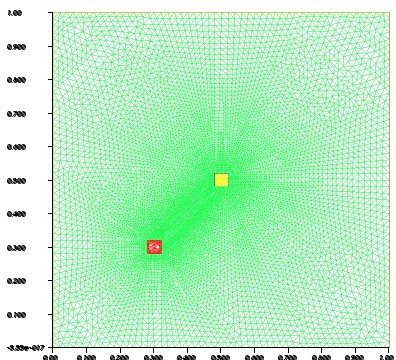
\includegraphics[width=0.3\textwidth]{mesh_test1.jpg}$
			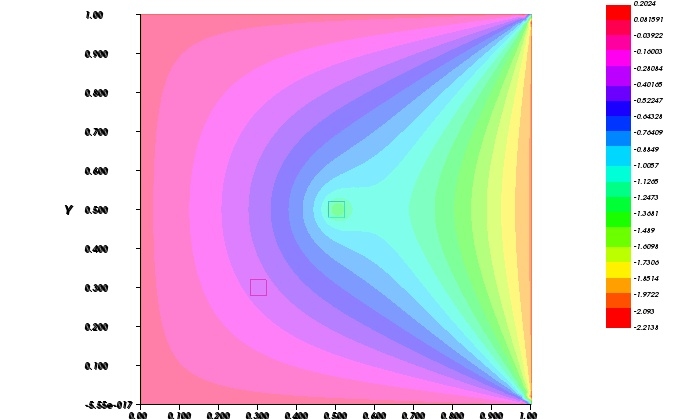
\includegraphics[width=0.3\textwidth]{pression_test1.jpg}$
			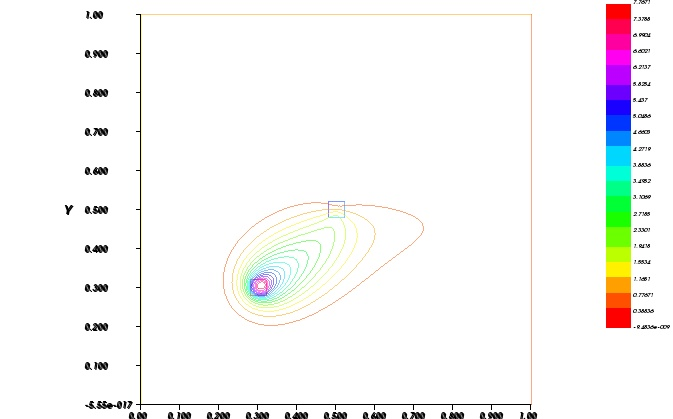
\includegraphics[width=0.3\textwidth]{pollutant_test1.jpg}
		\end{array}$
	\end{center}
	\caption{Non adaptive mesh on the left, pression in the center and diffusion of the pollutant on the right}
\end{figure} 
\subsection{Uniform refinement of the mesh}\label{splitmesh}
With this method we start from a mesh with triangles that is not forcedly the best, the general idea is that the first mesh has fewer triangles than we need, and we proceed to a generalised refinement of the mesh in all areas of the triangulation $\tau_h$ until a condition is respected. Since what we are interested in is the quantity of pollutant $c(\mathbf{x})$ pumped, in our case the stopping condition is achieved when the difference of the integral
\begin{equation}
	\int_{C_1} c(\mathbf{x})
\end{equation}
between two steps is less than a certain tolerance $TOL$. Since the value of the integral is of order $10^{-3}$ we take a tolerance $TOL=1\cdot 10^{-4}$
We obtain our goal in only 4 iterations. We start with a mesh of 1126 triangles and 584 vertices and after two split of the mesh we obtain a new mesh where every initial triangle $K$ is divided in eight sub-triangles, so the new mesh has 9008 triangles.\\ 
This type of mesh ensure us a good precision and has less elements, so the computation is clearly not as heavy as before.\\
The computed pollutant extracted by the pump by this method is 0.144219 cL. The result present a difference with the result of the other method.
\begin{figure}[h]
	\begin{center}$
		\begin{array}{ccc}
		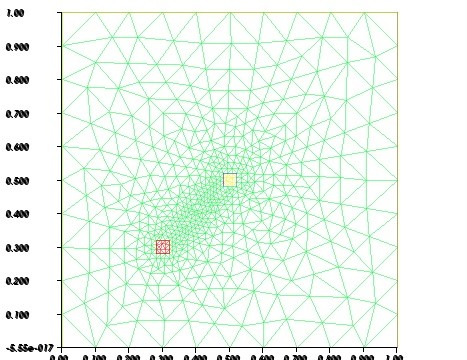
\includegraphics[width=0.3\textwidth]{adapt_mesh1.jpg}$
		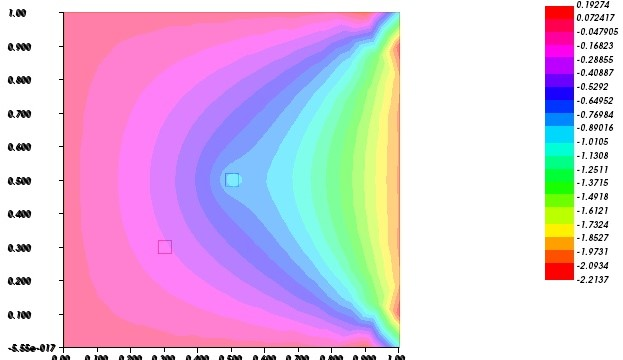
\includegraphics[width=0.3\textwidth]{pression1.jpg}$
		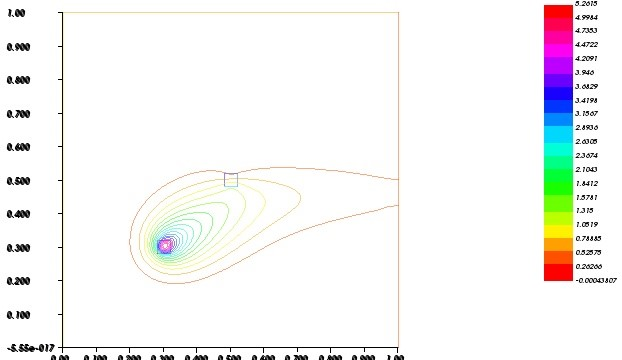
\includegraphics[width=0.3\textwidth]{pollution1.jpg}
		\end{array}$
	\end{center}
	\caption{Starting mesh for second and third methods, resulting pression and diffusion of the pollutant}
	\label{start23}
\end{figure} 
\begin{figure}
	\begin{center}$
		\begin{array}{ccc}
		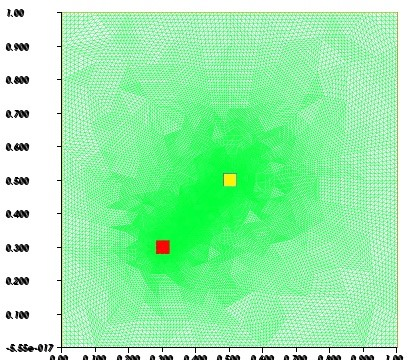
\includegraphics[width=0.3\textwidth]{adapt_mesh4.jpg}$
		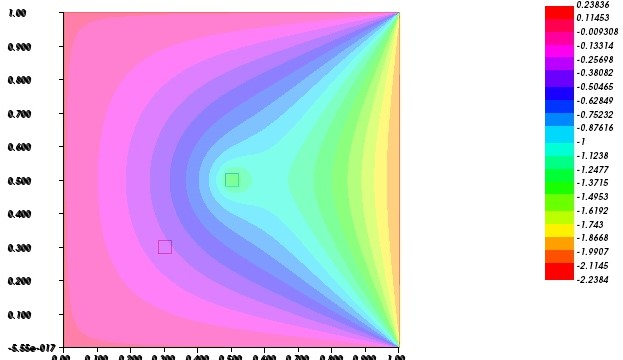
\includegraphics[width=0.3\textwidth]{pression4.jpg}$
		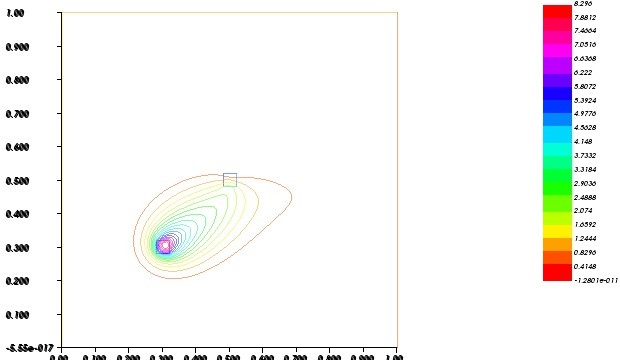
\includegraphics[width=0.3\textwidth]{pollution4.jpg}
		\end{array}$
	\end{center}
	\caption{Ending mesh for second method, resulting pression and diffusion of the pollutant}
	\label{end2}
\end{figure}
In the figure \ref{end2} we can see that the refinement of the mesh is generalised in all the domain $\Omega$, and a very different behaviour of the diffusion of the pollutant between the first (figure \ref{start23}) and the fourth step.
\subsection{Local refinement of the mesh}
The idea of this adaptive method is to refine the mesh only in the region we need a particular refinement in order to reach the same stopping condition as in section \ref{splitmesh}. To perform this task in FreeFem++ we use the command $adaptmesh(...)$. We start with the same mesh as in section \ref{splitmesh} in order to do a comparison between the two adaptive methods, a tolerance $TOL=0.001$ and an $h_max=0.1$, after each iteration these last two values will be divided by two. We reach the convergence condition after 2 iterations, when $TOL=0.0005$ and $h_max=0.05$, and the computed pumped pollutant is 0.151017 cL. An interesting remark that we can do is that also with this method we obtain another different value, this can be explained by the fact that the meshes used to compute these values are very different.
\begin{figure}
	\begin{center}$
		\begin{array}{ccc}
		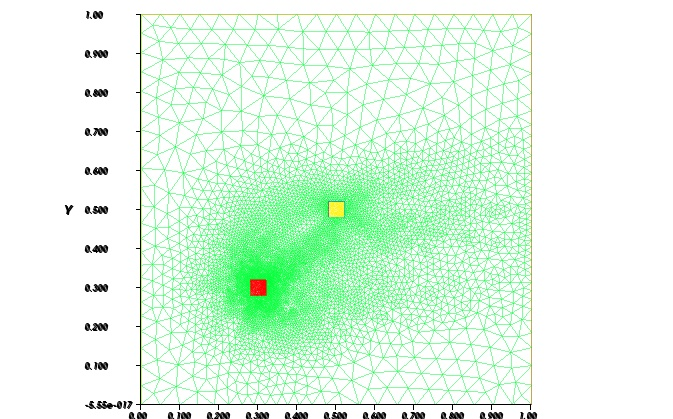
\includegraphics[width=0.3\textwidth]{mesh32.jpg}$
		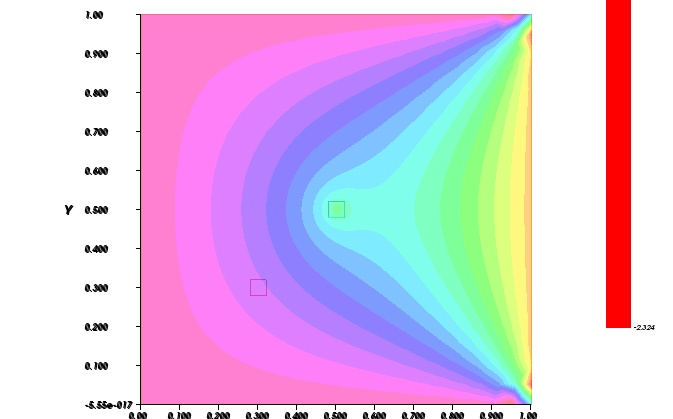
\includegraphics[width=0.3\textwidth]{pression32.jpg}$
		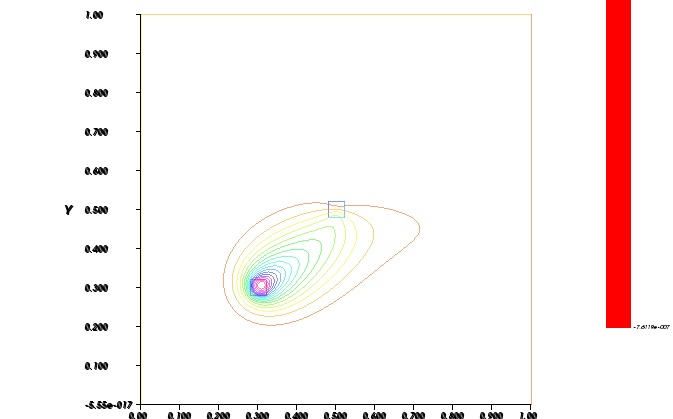
\includegraphics[width=0.3\textwidth]{pollutant32.jpg}
		\end{array}$
	\end{center}
	\caption{Ending mesh for third method, resulting pression and diffusion of the pollutant}
	\label{end3}
\end{figure} 
A particularity of the mesh in the figure \ref{end3} is the concentration of triangles in the area between area $C_1$ and $C_2$ but also a non refinement of the triangles near to the boundaries.
\subsection{comparison of the running time and convergence}
\begin{table}[h]
	\centering
	\caption{Running time of the methods}
	\label{run_time}
	\begin{tabular}{llll}
		Method & non adaptive & \begin{tabular}[c]{@{}l@{}}with\\ splitmesh\end{tabular} & \begin{tabular}[c]{@{}l@{}}with\\ adaptmesh\end{tabular} \\
		\begin{tabular}[c]{@{}l@{}}Running\\ Time\end{tabular} & 0.007 s & 0.008 s & 0.009 s
	\end{tabular}
\end{table}
As we can see in the table \ref{run_time} the running time of the three methods are not so different, but for the last two methods we have some guarantee of precision. Thus if we are obliged to choose a method it is preferable to choose one of the last two methods.\\
Finally I would dedicate this part to do a comparison of the quantity $\phi$.
\begin{figure}
	\begin{center}
		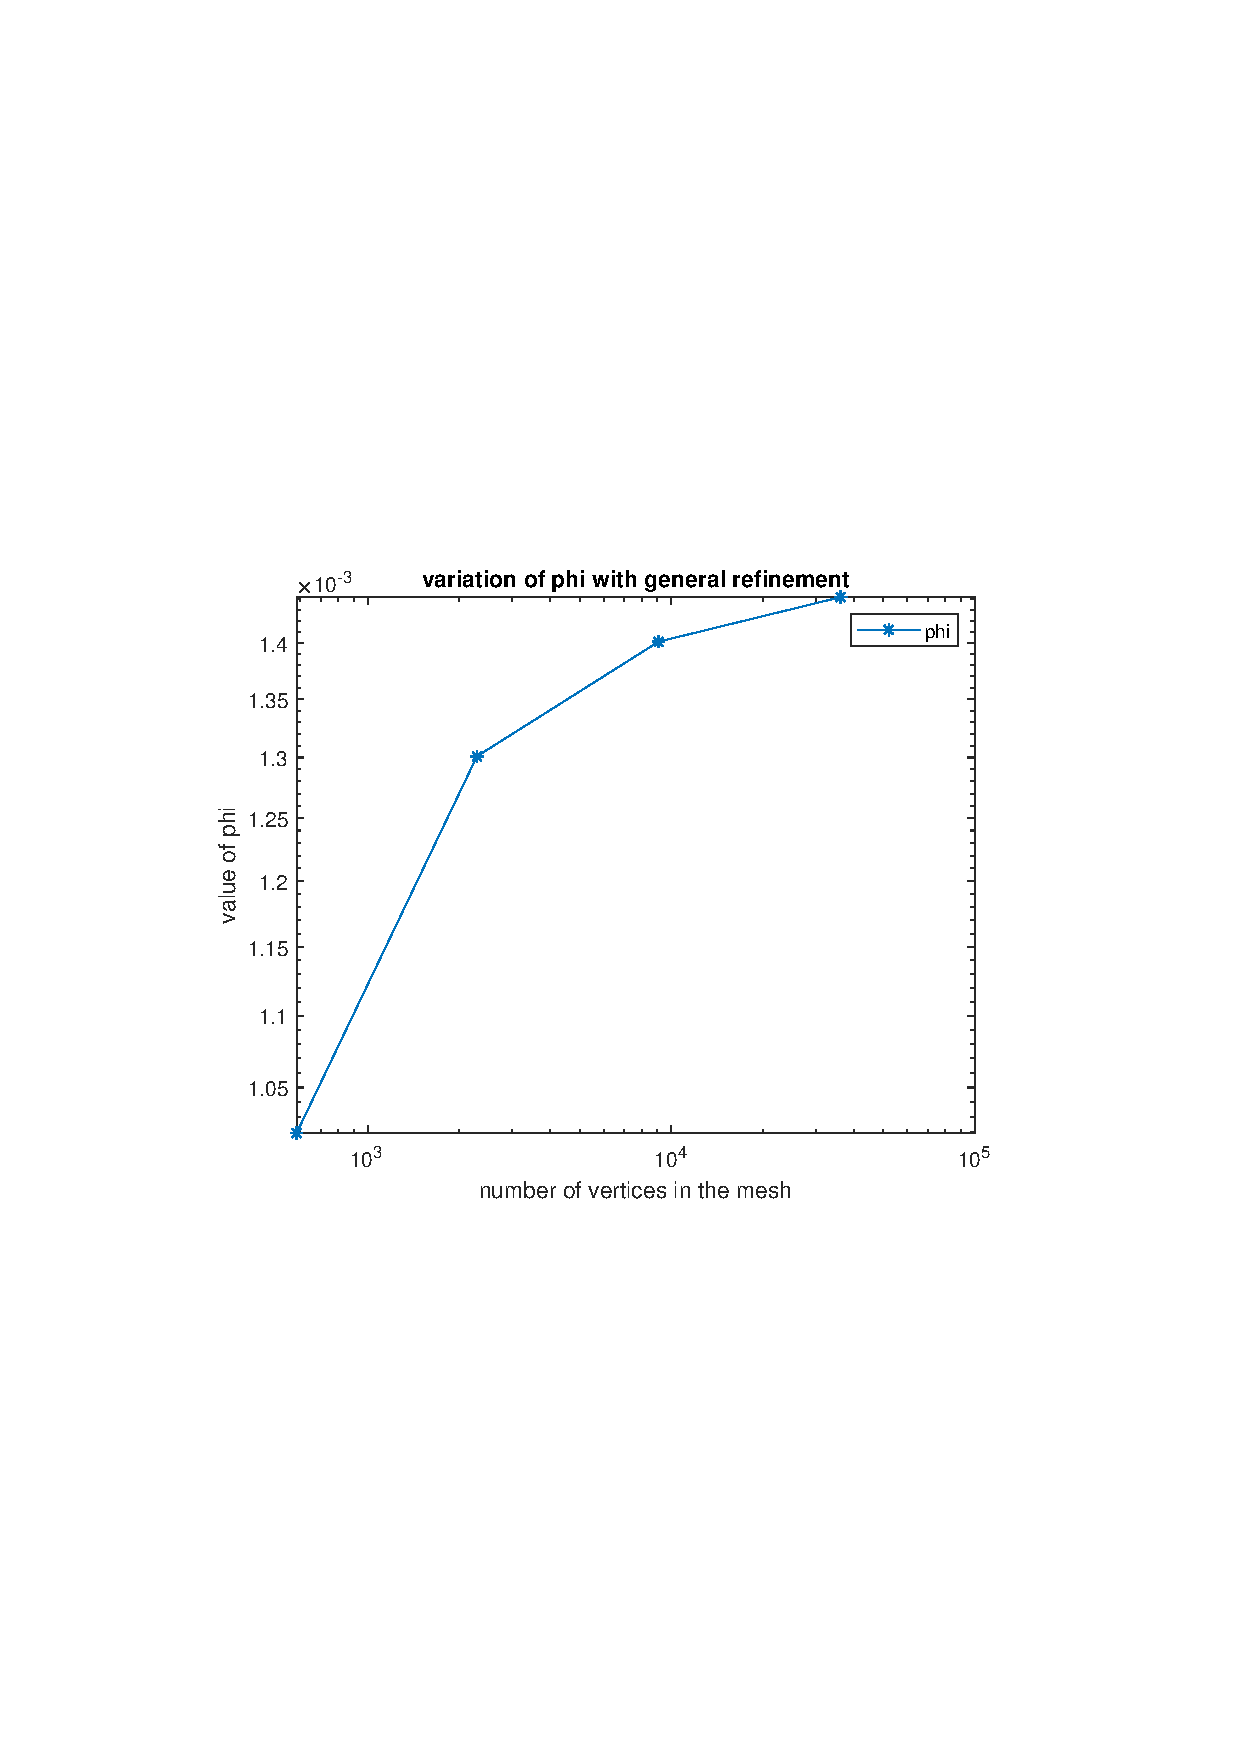
\includegraphics[width=0.45\textwidth]{plotphi_genref.pdf}
		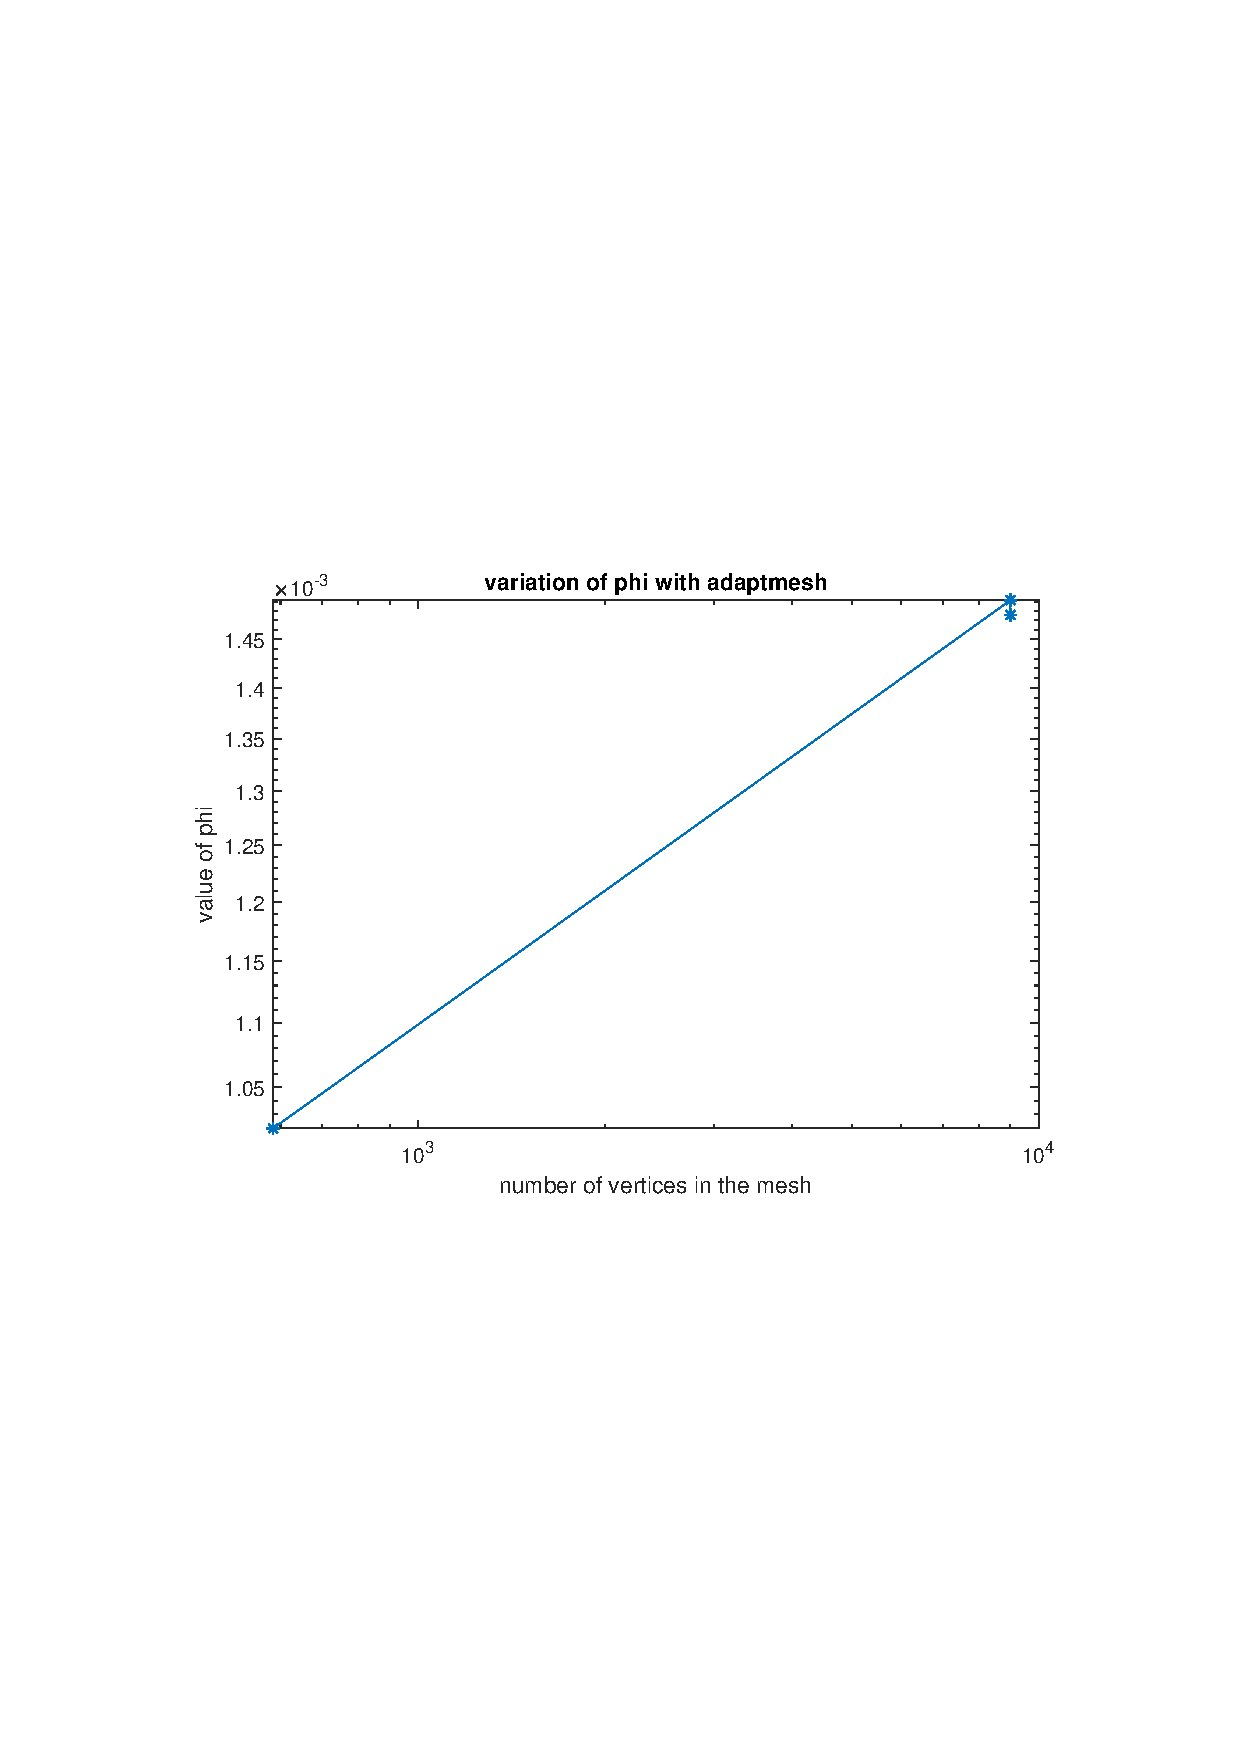
\includegraphics[width=0.45\textwidth]{plotphi_adapt.pdf}
	\end{center}
\caption{Plot in loglog scale of the variation of $\phi$}
\label{phi_comp}
\end{figure}
As we can see in the figure \ref{phi_comp} the convergence of the method with general refinement is slower then the other, indeed this method use 4 iterations and 10 times more vertices to obtain the same result that the method with local refinement can achieve in only 2 iterations.
\bibliography{biblio}
\bibliographystyle{plain}
\newpage
\appendix
\section{FreeFem++ code}
Here is my code for the three methods, there is no big difference between the three codes just some adjustment from a step to another.
\subsection{First method}
\lstset { %
	language=C++,
	backgroundcolor=\color{black!5}, % set backgroundcolor
	basicstyle=\footnotesize,% basic font setting
}
\begin{lstlisting}
	load "Element_Mixte"
	int tr=10;
	int tr1=50;
	real k=1;
	real pin=0;
	real pout=2;
	real nu=0.05;
	real phiv=5;
	macro div(v1,v2)(dx(v1)+dy(v2))//
	macro grad(p) [dx(p),dy(p)]//

	border a(t=0,1){x=t;y=0;label=1;};
	border b(t=0,1){x=1;y=t;label=2;};
	border c(t=1,0){x=t;y=1;label=3;};
	border d(t=1,0){x=0;y=t;label=4;};

	//region C1
	border a1(t=0.48,0.52){x=t;y=0.48;label=11;};
	border b1(t=0.48,0.52){x=0.52;y=t;label=12;};
	border c1(t=0.52,0.48){x=t;y=0.52;label=13;};
	border d1(t=0.52,0.48){x=0.48;y=t;label=14;};

	//regionC2
	border a2(t=0.28,0.32){x=t;y=0.28;label=21;};
	border b2(t=0.28,0.32){x=0.32;y=t;label=22;};
	border c2(t=0.32,0.28){x=t;y=0.32;label=23;};
	border d2(t=0.32,0.28){x=0.28;y=t;label=24;};

	mesh Th=buildmesh(a(tr1)+b(tr1)+c(tr1)+d(tr1)+a1(tr)
	+b1(tr)+c1(tr)+d1(tr)+a2(tr)+b2(tr)+c2(tr)+d2(tr));

	real phin=10;
	int r1=Th(0.5,0.5).region;
	int r2=Th(0.3,0.3).region;
	int r3=Th(0.7,0.7).region;
	fespace Qh(Th,P1);
	fespace Vh(Th,RT1);
	Qh f=-1000.*(region==r1)+0.*(region==r2)+0.*(region==r3);
	Qh g= 1000.*(region==r2)+0.*(region==r1)+0.*(region==r3);
	plot (Th);
	Qh ph,qh;
	Vh [uh1,uh2],[vh1,vh2];
	problem darcy([uh1,uh2,ph],[vh1,vh2,qh])=int2d(Th)(k^(-1)*
	(uh1*vh1+uh2*vh2))-
	int2d(Th)(qh*div(uh1,uh2))-
	int1d(Th,2)(pout*vh1)-
	int1d(Th,4)(-pin*vh1)-
	int2d(Th)(ph*div(vh1,vh2))+
	int2d(Th)(f*qh);
	darcy;
	plot(ph,fill=1,value=1,ps="pression_test1.jpg");

	fespace Wh(Th,P1);
	Wh ch,bh;
	problem	transport(ch,bh)=int2d(Th)(nu*(dx(ch)*dx(bh)+dy(ch)*
	dy(bh)))+
	int2d(Th)((uh1*dx(ch)+uh2*dy(ch))*bh)-
	int2d(Th)(g*bh)+on(1,3,4, ch=0);
	transport;
	plot(ch,value=1,ps="pollutant_test1.jpg");
	phin=int2d(Th,r1)(ch);

	cout<<phin<<endl;

\end{lstlisting}
\subsection{Second method}
\begin{lstlisting}
	load "Element_Mixte"
	real tol=0.0001;
	real k=1;
	real pin=0;
	real pout=2;
	real nu=0.05;
	real phin=10;
	real phiv=5;
	int i=1;
	macro div(v1,v2)(dx(v1)+dy(v2))//
	macro grad(p) [dx(p),dy(p)]//
	
	border a(t=0,1){x=t;y=0;label=1;};
	border b(t=0,1){x=1;y=t;label=2;};
	border c(t=1,0){x=t;y=1;label=3;};
	border d(t=1,0){x=0;y=t;label=4;};
	
	//region C1
	border a1(t=0.48,0.52){x=t;y=0.48;label=11;};
	border b1(t=0.48,0.52){x=0.52;y=t;label=12;};
	border c1(t=0.52,0.48){x=t;y=0.52;label=13;};
	border d1(t=0.52,0.48){x=0.48;y=t;label=14;};
	
	//regionC2
	border a2(t=0.28,0.32){x=t;y=0.28;label=21;};
	border b2(t=0.28,0.32){x=0.32;y=t;label=22;};
	border c2(t=0.32,0.28){x=t;y=0.32;label=23;};
	border d2(t=0.32,0.28){x=0.28;y=t;label=24;};
	
	mesh Th=buildmesh(a(10)+b(10)+c(10)+d(10)+
	a1(3)+b1(3)+c1(3)+d1(3)+a2(3)+b2(3)+c2(3)+d2(3));
	
	while(abs(phin-phiv)>tol)
	{
	phiv=phin;
	int r1=Th(0.5,0.5).region;
	int r2=Th(0.3,0.3).region;
	int r3=Th(0.7,0.7).region;
	fespace Qh(Th,P1);
	fespace Vh(Th,RT1);
	Qh f=-1000.*(region==r1)+0.*(region==r2)+0.*(region==r3);
	Qh g= 1000.*(region==r2)+0.*(region==r1)+0.*(region==r3);
	plot (Th);
	Qh ph,qh;
	Vh [uh1,uh2],[vh1,vh2];
	problem darcy([uh1,uh2,ph],[vh1,vh2,qh])=int2d(Th)
	(k^(-1)*(uh1*vh1+uh2*vh2))-
	int2d(Th)(qh*div(uh1,uh2))-
	int1d(Th,2)(pout*vh1)-
	int1d(Th,4)(-pin*vh1)-
	int2d(Th)(ph*div(vh1,vh2))+
	int2d(Th)(f*qh);
	darcy;
	plot(ph,fill=1, value=1,coef=1);
	
	fespace Wh(Th,P1);
	Wh ch,bh;
	problem transport(ch,bh)=int2d(Th)
	(nu*(dx(ch)*dx(bh)+dy(ch)*dy(bh)))+
	int2d(Th)((uh1*dx(ch)+uh2*dy(ch))*bh)-
	int2d(Th)(g*bh)+on(1,3,4, ch=0);
	transport;
	plot(ch,value=1,fill=0);
	phin=int2d(Th,r1)(ch);
	Th=splitmesh(Th,2);
	cout<<phin<<endl;
	i=i+1;
	}
\end{lstlisting}
\subsection{Third method}
\begin{lstlisting}
	load "Element_Mixte"
	real tol=0.002;
	real h=0.1;
	real k=1;
	real pin=0;
	real pout=2;
	real nu=0.05;
	real phin=10;
	real phiv=5;
	int i=1;
	macro div(v1,v2)(dx(v1)+dy(v2))//
	macro grad(p) [dx(p),dy(p)]//
	
	border a(t=0,1){x=t;y=0;label=1;};
	border b(t=0,1){x=1;y=t;label=2;};
	border c(t=1,0){x=t;y=1;label=3;};
	border d(t=1,0){x=0;y=t;label=4;};
	
	//region C1
	border a1(t=0.48,0.52){x=t;y=0.48;label=11;};
	border b1(t=0.48,0.52){x=0.52;y=t;label=12;};
	border c1(t=0.52,0.48){x=t;y=0.52;label=13;};
	border d1(t=0.52,0.48){x=0.48;y=t;label=14;};
	
	//regionC2
	border a2(t=0.28,0.32){x=t;y=0.28;label=21;};
	border b2(t=0.28,0.32){x=0.32;y=t;label=22;};
	border c2(t=0.32,0.28){x=t;y=0.32;label=23;};
	border d2(t=0.32,0.28){x=0.28;y=t;label=24;};
	
	mesh Th=buildmesh(a(10)+b(10)+c(10)+d(10)
	+a1(3)+b1(3)+c1(3)+d1(3)+a2(3)+b2(3)+c2(3)+d2(3));
	
	while(abs(phin-phiv)>tol)
	{
	tol=tol/2;
	h=h/2;
	phiv=phin;
	int r1=Th(0.5,0.5).region;
	int r2=Th(0.3,0.3).region;
	int r3=Th(0.7,0.7).region;
	fespace Qh(Th,P1);
	fespace Vh(Th,RT1);
	Qh f=-1000.*(region==r1)+0.*(region==r2)+0.*(region==r3);
	Qh g= 1000.*(region==r2)+0.*(region==r1)+0.*(region==r3);
	plot (Th,ps="mesh3"+i+".jpg");
	Qh ph,qh;
	Vh [uh1,uh2],[vh1,vh2];
	problem darcy([uh1,uh2,ph],[vh1,vh2,qh])=int2d(Th)
	(k^(-1)*(uh1*vh1+uh2*vh2))-
	int2d(Th)(qh*div(uh1,uh2))-
	int1d(Th,2)(pout*vh1)-
	int1d(Th,4)(-pin*vh1)-
	int2d(Th)(ph*div(vh1,vh2))+
	int2d(Th)(f*qh);
	darcy;
	plot(ph,fill=1, value=1,coef=1,ps="pression3"+i+".jpg");
	
	fespace Wh(Th,P1);
	Wh ch,bh;
	problem transport(ch,bh)=int2d(Th)
	(nu*(dx(ch)*dx(bh)+dy(ch)*dy(bh)))+
	int2d(Th)((uh1*dx(ch)+uh2*dy(ch))*bh)-
	int2d(Th)(g*bh)+on(1,3,4, ch=0);
	transport;
	plot(ch,value=1,fill=0,ps="pollutant3"+i+".jpg");
	phin=int2d(Th,r1)(ch);
	Th=adaptmesh(Th,err=tol,hmax=h,iso=1,ch);
	cout<<phin<<endl;
	i=i+1;
	}
\end{lstlisting}
\end{document}   
       
